\documentclass{beamer}
\usepackage[utf8]{inputenc}
\usetheme{Warsaw}
\title[Datalogi i uddannelsen]{Datalogi i uddannelsen}
\author{Mikkel Kragh, Jannik Gram, Rune Abrahamsson, Rasmus Abrahamsen}
\institute{DIKU}
\date{\today}
\begin{document}

\begin{frame}
\titlepage
\end{frame}


\begin{frame}{Problemet}
\begin{itemize}
\item Stigende brug af computere.
\item Uoptimalt brug i forhold til behov. F.eks.
\begin{itemize}
\item Word + email til samarbejde.
\item Windows
\end{itemize}
\end{itemize}

\end{frame}

\begin{frame}{Datalogi i folkeskolen}

\begin{itemize}
\item Der skal indføres datalogi i folkeskolen.
\item Men er der tid nok?
\item Det kan der blive. Mere ubrugelige fag som kemi og fysik skal give plads til datalogi.
\end{itemize}


\includegraphics[width=60mm]{skole.png}

\end{frame}

\begin{frame}{Datalogi i gymnasiet}
I gymnasiet vil eleverne kunne skrive rapporter og afleveringer i LaTeX og kollaborere vha. værktøjer som for eksempel git.

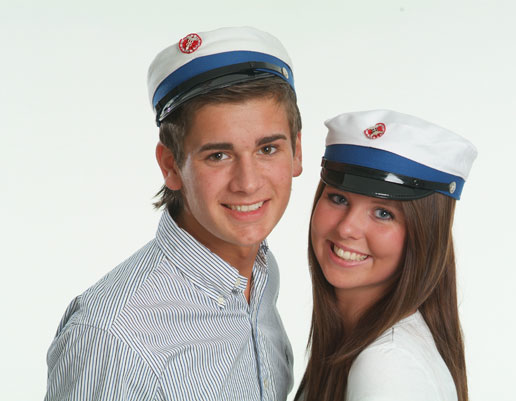
\includegraphics[width=60mm]{gymnasie.png}

\end{frame}

\begin{frame}{Undervisningsform}
\begin{itemize}
\item Selvstændigt fag
\begin{itemize}
\item Fokus på datalogisk tænkning
\item Dedikeret lærer/vidensbase
\end{itemize}
\item Som del af andre fag
\begin{itemize}
\item Fokus på datalogi som redskab
\item Større integration
\end{itemize}
\end{itemize}
\end{frame}

\begin{frame}{Perspektivering}

Om nogle år bliver det nice.

\end{frame}

\begin{frame}{TAK}

\end{frame}


\end{document}
